\chapter{Resultados y Análisis}

En este capítulo se presentan los resultados obtenidos de la implementación
del sistema. Se comienza presentando los resultados obtenidos por el
extractor de información y presentando la base de datos de \textit{embeddings}
generada. A continuación, se muestra el conjunto de datos de preguntas
y respuestas generado, así como los resultados de las
evaluaciones de los diferentes modelos de extracción de \textit{embeddings}
y de inferencia de respuestas. Posteriormente, se presentan
los resultados del reentrenamiento de los modelos de \textit{embeddings},
para finalmente describir el proceso de puesta en producción del sistema.
En cada paso se discutirán los resultados mostrados, así como los retos y
criterios considerados en la toma de decisiones que llevaron a la
configuración final del sistema en producción. Finalmente, se presenta un
análisis general del sistema.

\section{Extractor de información}

En la metodología se mencionan dos formas de extraer la información de los
documentos normativos, usando \textit{PyPdf+PyTesseract} y empleando
\textit{Pdfplumber}. Ambos métodos cumplieron con la finalidad generar una
base de datos de \textit{embeddings} con toda la información de los
documentos normativos, incluyendo la estrutura de los documentos con
sus títulos y secciones. Sin embargo, \textit{Pdfplumber} mostró mayores
ventajas, por lo que se seleccionó como método de extracción de información
en el sistema final.
En las siguientes subsecciones se presentan algunas de las consideraciones
adicionales que se tuvieron que implementar para hacer la correcta
extracción de la información así como el razonamiento para seleccionar
\textit{Pdfplumber} sobre \textit{PyPdf+PyTesseract}.

\subsection{Eliminación de encabezados y pies de página}

Todos los documentos normativos de la universidad tienen un encabezado con
el nombre del documento y un pie de página con el número de página, esta es
información irrelevante que se desea eliminar. Para eliminar estos elementos
se normalizó a 1.0 el ancho y alto de la página, para posteriormente
establecer los márgenes superior, inferior, izquierdo y derecho.
Todo el texto que se encuentre fuera de dichos márgenes es ignorado como
se muestra en la Figura \ref{fig:quitar_encabezados}. El ancho y alto totales
del documento se obtienen directamente de \textit{PyPdf}, \textit{PyTesseract}
o \textit{Pdfplumber} según sea el caso. La mayoría de los documentos normativos
comparten un márgen de: (izquierda: 0.5, arriba: 0.1, derecha: 0.95, abajo: 0.95),
sin embargo, este parámetro es configurable mediante un archivo YAML para
dar flexibilidad al procesar documentos con márgenes diferentes.

\begin{figure}
    \centering
    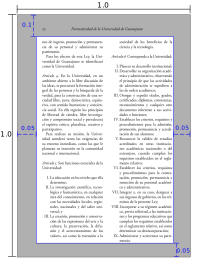
\includegraphics[width = 0.8\textwidth]{\DirFigCcuatro/quitar_encabezados}
    \caption{Elminación de encabezados y pies de página con márgenes.}
    \label{fig:quitar_encabezados}
\end{figure}

\subsection{Detección de títulos centrados}

Inicialmente, la detección de títulos centrados se realizó línea por línea,
para no tener que detectar los bloques separados verticalmente,
sin embargo, hay ocasiones en las que la línea parece estar centrada
(recuadro rojo de Figura \ref{fig:titulo_wrong}), cuando en realidad
es parte de una viñeta o de un texto con sangría, es por ello que es
necesario hacer el análisis por bloques separados verticalmente
(recuadro verde de Figura \ref{fig:titulo_wrong}).
Se determina que un bloque está separado verticalmente cuando hay una distancia
mayor a un valor configurable, proporcional al alto de la línea como se
muestra en la Figura \ref{fig:titulo_ok}.

\begin{figure}
    \centering
    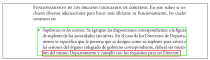
\includegraphics[width = 0.8\textwidth]{\DirFigCcuatro/title_wrong}
    \caption{Línea de texto aparentemente centrada (recuadro rojo) que al
        separar el documento en bloques (recuadro verde) ya no se detecta como título.}
    \label{fig:titulo_wrong}
\end{figure}

\begin{figure}
    \centering
    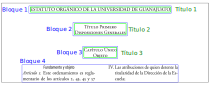
\includegraphics[width = 0.8\textwidth]{\DirFigCcuatro/title_ok}
    \caption{Detección correcta de títulos centrados y agrupación en bloques de texto
        por separación vertical.}
    \label{fig:titulo_ok}
\end{figure}

De la misma forma, inicialmente se planteó identificar los títulos
centrados en la columna analizando línea por línea, sin embargo, cuando
el texto es muy extenso, ya no parece estar centrado, como en la Figura
\ref{fig:title_column}. Por lo anterior, se recurrió al mismo enfoque donde
se detecta el bloque de texto y se da una tolerancia de $L$ líneas para
detectar el inicio de un artículo con la expresión regular, de ser así,
las $l$ líneas previas son consideradas como un título del artículo.

\begin{figure}
    \centering
    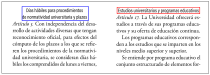
\includegraphics[width = 0.8\textwidth]{\DirFigCcuatro/title_column}
    \caption{Título centrado en columna ideal (izquierda) y título centrado en
        columna que no puede ser detectado como texto centrado (derecha).}
    \label{fig:title_column}
\end{figure}

\subsection{Detección de títulos no centrados}

El documento correspondiente al modelo educativo de la
universidad, rompe con la estructura de los demás documentos, pues no es un
documento con artículos, sino más bien una guía de la estructura educativa
de la institución. Esto no impide que sea dividido en secciones y fragmentos,
pero difiere en que el texto está justificado a una columna y
sus secciones son numéricas y sin centrar. Para detectar estas secciones no centradas,
el texto se divide en bloques verticales y cada bloque se valida
con una expresión regular como se muestra en la Figura \ref{fig:titulo_no_centrado}.
Esta validación no interfiere con la detección de títulos centrados
pues ambos procesos se realizan para todos los documentos.

\begin{figure}
    \centering
    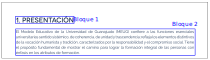
\includegraphics[width = 0.8\textwidth]{\DirFigCcuatro/titulo_no_centrado}
    \caption{Documento con títulos a la izquierda son detectados al separalos
        en bloques verticales y validar contra una expresión regular.}
    \label{fig:titulo_no_centrado}
\end{figure}

\subsection{Generación del árbol}

La generación del árbol con la estructura del documento se realizó
adecuadamente para todos los documentos normativos, sin embargo, se detectó
que al generar la estructura del preámbulo de los documentos,
ésta puede presentar algunas estructuras poco
congruentes, como se observa en el recuadro rojo de la Figura
\ref{fig:arbol}. Sin embargo, estas estructuras no afectan el sistema
pues la estructura de capítulos y artículos se genera correctamente,
como se observa en el recuadro verde de la Figura \ref{fig:arbol}, además
el preámbulo puede ignorarse si así se deseara pues no contiene información
relevante para la normativa en la mayoría de los casos. Adicionalmente, en la Figura
\ref{fig:arbol_2} se muestra parte de la estructura generada para el documento
``Modelo Educativo de la Universidad de guanajuato y su Modelo Académico''
que, a pesar de que el documento tiene una estructura diferente, puede
procesarse adecuadamente.

\begin{figure}
    \centering
    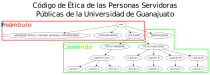
\includegraphics[width = 0.8\textwidth]{\DirFigCcuatro/arbol}
    \caption{Árbol de documento generado automáticamente. Se observa el preámbulo
        con algunos títulos erroneos (recuadro rojo) y el contenido del documento
        detectado correctamente (recuadro verde).}
    \label{fig:arbol}
\end{figure}

\begin{figure}
    \centering
    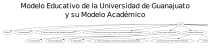
\includegraphics[width = 0.8\textwidth]{\DirFigCcuatro/arbol_2}
    \caption{Árbol de documento ``Modelo Educativo de la Universidad de guanajuato y su Modelo Académico''
        que es un documento a una columna, justificado y con secciones numéricas.}
    \label{fig:arbol_2}
\end{figure}

\subsection{Separación en fragmentos}

Al generar el árbol del documento, colocando un artículo en cada nodo, se encontró
que hay artículos cuya longitud superan los 10,000 caracteres, lo cual
provoca que la cantidad de recursos necesarios para procesarlos enteros sea muy grande.
Es por ello que se hicieron múltiples pruebas para seleccionar
el número máximo de caracteres por fragmento en que se debía dividir cada nodo.
Estas pruebas consideraron la VRAM disponible, la longitud media y máxima del
contenido de los nodos, entre otros factores. Al final, se encontró que se pueden
usar adecuadamente los modelos de \textit{embeddings} con 2,048 tokens de contexto, lo que
equivale a aproximadamente 8,200 caracteres si se usa el tokenizador de Qwen 3.
Por lo anterior, el límite de caracteres por fragmento se estableció en 8,000,
ya que al dividirse por párrafos el fragmento más grande resultó de 1,964 tokens.

\subsection{Detección de tablas}

Un problema que no se pudo resolver durante la implementación de esta herramienta
es la detección de tablas en los documentos. Una tabla es un elemento que puede
ser complejo, especialmente cuando cada celda es de más de un renglón o
se mezclan alineaciones de las columnas, todo esto hace que los extractores de
texto, tanto \textit{PyPDF}, \textit{PyTesseract} y \textit{Pdfplumber} desorganicen
el texto de las tablas, generando secuencias ilegibles como se muestra en la Figura
\ref{fig:tablas_1}. Este proceso se acentúa más cuando las tablas están
orientadas verticalmente, en lugar de horizontalmente, como es el caso de
uno de los documentos de la normativa. Dada esta circunstancia, las partes
del documento con tablas verticales fueron eliminadas completamente y las
otras tablas que aparecen en los documentos fueron dejadas como están.

\begin{figure}
    \centering
    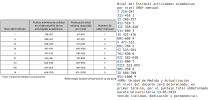
\includegraphics[width = 0.8\textwidth]{\DirFigCcuatro/tablas_1}
    \caption{Extracción de tabla como texto. A la izquierda se muestra la tabla
        original y a la derecha la secuencia de texto desorganizado.}
    \label{fig:tablas_1}
\end{figure}

\subsection{\textit{PyPDF+PyTesseract} y Pdfplumber}

En general, ambas metodologías fueron capaces de extraer los árboles con la
estructura de los documentos PDF, así como su contenido, sin embargo,
el enfoque de \textit{PyPDF+PyTesseract} es mucho más lento, pues tarda
5 minutos en procesar un documento de 48 páginas, mientras
que \textit{Pdfplumber} demora 45 segundos. En un intento de reducir
el tiempo de procesamiento se paralelizó el procesamiento de las páginas,
logrando reducir a 2.5 minutos al procesar 4 páginas en paralelo, pudiendo
disminuir más con más núcleos de procesamiento. Otra
desventaja de \textit{PyPDF+PyTesseract} es que se encontró texto no visible
en los documentos PDF de la normativa, especialmente palabras que al obtener
el texto plano con \textit{PyPDF} se duplican o triplican como se muestra
en la Figura \ref{fig:texto_duplicado}, lo cual altera
considerablemente el algoritmo y requiere de un proceso adicional para
eliminarlas, este proceso se puede hacer directamente con \textit{Pdfplumber}
con una bandera de configuración. Sin embargo, una bentaja de
\textit{PyPDF+PyTesseract} es que permite al sistema detectar texto escrito en
imágenes, aunque en toda la normativa solamente hay un documento que lo tiene
y es en su portada, la cual puede simplemente ser ignorada. En la Tabla
\ref{tab:mixed_vs_pdfplumber} se muestra una comparación entre ambos métodos,
donde se observa que emplear únicamente \textit{Pdfplumber} es más beneficioso
para el tipo de documentos de la normativa de la universidad.

\begin{figure}
    \centering
    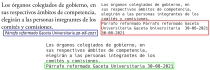
\includegraphics[width = 0.8\textwidth]{\DirFigCcuatro/texto_duplicado}
    \caption{Ejemplo de texto oculto. (Arriba a la izquierda) Párrafo como aparece en archivo
        PDF. (Arriba a la derecha) Texto extraído con \textit{PyPDF}. (Abajo al centro)
        Texto corregido sin texto duplicado.}
    \label{fig:texto_duplicado}
\end{figure}

\begin{table}[!ht]
    \centering
    \begin{tabular}{|l|l|l|}
        \hline
        Característica           & \textit{PyPDF+PyTesseract} & \textit{Pdfplumber} \\ \hline
        Tiempo de procesamiento  & 3.12 s/pag                 & \textbf{0.93 s/pag} \\ \hline
        Texto en imágenes        & \textbf{SÍ}                & NO                  \\ \hline
        Almacenamiento adicional & SÍ                         & \textbf{NO}         \\ \hline
    \end{tabular}
    \caption{Tabla comparativa de métodos de extracción de información. Pruebas
        realizadas en computadora con un procesador Intel\textregistered Core\textregistered i5-8300H CPU @ 2.30GHz}
    \label{tab:mixed_vs_pdfplumber}
\end{table}

\section{Conjunto de datos generado}

El conjunto de datos que se generó recopila preguntas y respuestas de
21 documentos diferentes, con un total de 1,082 preguntas y respuestas,
la distribución de preguntas por cada documento se muestra en la Figura
\ref{fig:dataset_questions}. Un ejemplo de un registro del conjunto de
datos generado se ve como el siguiente:

\begin{itemize}
    \item \textbf{id:} 81e729afa369916be4d4db99f9c1817c
    \item \textbf{title:} ley-organica-de-la-universidad-de-guanajuato
    \item \textbf{context:} Artículo 1
    \item \textbf{context\_text:} La presente Ley es de orden público y de interés social. Contiene las normas fundamentales de la misión, organización, funcionamiento y gobierno de la Universidad de Guanajuato.
    \item \textbf{question:} ¿Qué contiene la Ley Orgánica de la Universidad de Guanajuato?
    \item \textbf{answers:} \{'text': ['Contiene las normas fundamentales de la misión, organización, funcionamiento y gobierno de la Universidad de Guanajuato']\}
\end{itemize}

\begin{figure}[]
    \centering
    \includegraphics[width = 0.8\textwidth]{\DirFigCcuatro/dataset_questions}
    \caption{Distribución de preguntas por documento.}
    \label{fig:dataset_questions}
\end{figure}

Durante la generación del conjunto de datos se observaron varias particularidades
de los documentos que se tomaron en cuenta para generar las preguntas y se
deberán tener en consideración durante la evaluación de los modelos.
No fue posible generar preguntas concretas del preámbulo de los documentos,
por lo que estas partes fueron omitidas. Otro elemento particular es la
presencia de artículos transitorios, los cuales, como su nombre lo indica,
son de caracter temporal y solo tienen relevancia cuando recién se publica el
documento o la reforma al documento, por lo que incluirlos podría ser
inecesario o contradictorio, pues muchos hacen referencia
a fechas o tiempos de los cuales el sistema no tiene conocimiento. A pesar
de esto, todas las pruebas se realizaron incluyendo estos artículos.

Adicionalmente, en el conjunto de datos se observa cierta tendencia a
que las preguntas contengan las palabras clave al cual están redactadas
en los artículos, usando el nombre completo y apropiado para cada elemento,
ej: ¿Cuáles son las responsabilidades de la persona titular de la Rectoría
General?, cuando sería más natural preguntar ¿Cuáles son las responsabilidades
del Rector General?. Esto podría generar pregunta más fáciles de responder y
con lenguaje un poco alejado del lenguaje común del usuario final.

Una vez recopiladas las preguntas y respuestas, el conjunto
de datos se dividió en dos subconjuntos: entrenamiento
(80\%) y prueba (20\%). El objetivo de esta división es emplear el conjunto de prueba
durante la evaluación de los modelos de \textit{embeddings} reentrenados,
sin embargo, para las demás evaluaciones se empleó el conjunto de datos
completo para evaluar. El conjunto de datos se colocó en un repositorio de
HuggingFace con el objetivo de facilitar su uso en los diferentes equipos
de trabajo, así como su publicación. Usar esta estrategia demostró ser
efectiva pues se pueden conservar diferentes versiones del conjunto de
datos de forma organizada, así como los subconjuntos de entrenamiento y prueba.

\section{Evaluación y selección del modelo de \textit{embeddings}}

Se evaluaron tres modelos diferentes: MiniLM, MPNET y Qwen 3. Del modelo
Qwen 3 se evaluaron sus tres variantes de tamaño: 0.6B, 4B y 8B, para
cada variante se evaluó además su versión cuantizada disponible más pequeña y
la más grande. Adicionalmente, se evaluaron los modelos con k=3 y k=5
fragmentos similares, dando como resultados los mostrados en las Tablas
\ref{tab:metrics_embedding_top_3} y \ref{tab:metrics_embedding_top_5} para
top-3 y top-5 de fragmentos similares respectivamente. Se debe considerar que la precisión
y la puntuación f1 son naturalmente bajos puesto que cada pregunta del conjunto
de datos fue formulada para que tenga un solo artículo relevante, es decir,
el máximo de fragmentos relevantes por pregunta es 1 o 2 (dado que unos pocos
artículos son de más de un fragmento), de ahí que la mejor
métrica para comparar los modelos sea únicamente el recall.

Si se compara el recall (Figuras
\ref{fig:metrics_embedding_top_3}, \ref{fig:metrics_embedding_top_5}), se
puede observar que el mejor modelo es el Qwen3-Embedding-8B, seguido de sus
versiones cuantizadas. Este resultado nos permite seleccionar al modelo
Qwen-Embedding-8B para las siguientes pruebas, así como a su modelo
cuantizado Q4\_K\_M de 4 bits, que con mucha menos memoria alcanza un
rendimiento similar. Por otra parte, se observa la considerable diferencia
de 0.63 y 0.5 puntos de recall entre el mejor modelo y los modelos
all-MiniLM-L6-v2 y multi-qa-mpnet-base-dot-v1 respectivamente. Además,
observamos que existe una diferencia de aproximadamente 0.8 puntos entre
las pruebas con el top-5 de fragmentos similares respecto al top-3, esto es indicativo
de que no siempre el fragmento relevante real está dentro de de los tres
fragmentos más similares, por
lo que alimentar el modelo de inferencia con 5 fragmentos de contexto entregará
mejores resultados sacrificando un poco de memoria para el contexto.

\begin{table}[!ht]
    \centering
    \begin{tabular}{|l|l|l|l|}
        \hline
        Modelo de \textit{embeddings} & precision@3    & recall@3       & f1@3           \\ \hline
        Qwen3-Embedding-0.6B          & 0.184          & 0.549          & 0.274          \\ \hline
        Qwen3-Embedding-0.6B-f16      & 0.248          & 0.743          & 0.371          \\ \hline
        Qwen3-Embedding-0.6B-Q8\_0    & 0.247          & 0.738          & 0.369          \\ \hline
        Qwen3-Embedding-4B            & 0.195          & 0.584          & 0.292          \\ \hline
        Qwen3-Embedding-4B-Q4\_K\_M   & 0.283          & 0.843          & 0.422          \\ \hline
        Qwen3-Embedding-4B-f16        & 0.282          & 0.841          & 0.420          \\ \hline
        \textbf{Qwen3-Embedding-8B}   & \textbf{0.304} & \textbf{0.909} & \textbf{0.454} \\ \hline
        Qwen3-Embedding-8B-Q4\_K\_M   & 0.285          & 0.852          & 0.426          \\ \hline
        Qwen3-Embedding-8B-f16        & 0.286          & 0.855          & 0.427          \\ \hline
        all-MiniLM-L6-v2              & 0.091          & 0.273          & 0.136          \\ \hline
        multi-qa-mpnet-base-dot-v1    & 0.133          & 0.400          & 0.200          \\ \hline
    \end{tabular}
    \caption{Resultados de evaluación para modelos de \textit{embeddings} con el top-3 de fragmentos similares.}
    \label{tab:metrics_embedding_top_3}
\end{table}

\begin{table}[!ht]
    \centering
    \begin{tabular}{|l|l|l|l|}
        \hline
        Modelo de \textit{embeddings} & precision@5    & recall@5       & f1@5  \\ \hline
        Qwen3-Embedding-0.6B          & 0.128          & 0.637          & 0.212 \\ \hline
        Qwen3-Embedding-0.6B-Q8\_0    & 0.169          & 0.840          & 0.280 \\ \hline
        Qwen3-Embedding-0.6B-f16      & 0.169          & 0.840          & 0.280 \\ \hline
        Qwen3-Embedding-4B            & 0.137          & 0.681          & 0.227 \\ \hline
        Qwen3-Embedding-4B-Q4\_K\_M   & 0.186          & 0.919          & 0.306 \\ \hline
        Qwen3-Embedding-4B-f16        & 0.185          & 0.917          & 0.305 \\ \hline
        \textbf{Qwen3-Embedding-8B}   & \textbf{0.198} & \textbf{0.986} & 0.329 \\ \hline
        Qwen3-Embedding-8B-Q4\_K\_M   & 0.185          & 0.919          & 0.306 \\ \hline
        Qwen3-Embedding-8B-f16        & 0.187          & 0.928          & 0.309 \\ \hline
        all-MiniLM-L6-v2              & 0.071          & 0.356          & 0.118 \\ \hline
        multi-qa-mpnet-base-dot-v1    & 0.099          & 0.493          & 0.164 \\ \hline
    \end{tabular}
    \caption{Resultados de evaluación para modelos de \textit{embeddings} con el top-5 de fragmentos similares.}
    \label{tab:metrics_embedding_top_5}
\end{table}

\begin{figure}
    \centering
    \includegraphics[width = 0.8\textwidth]{\DirFigCcuatro/metrics_embedding_top_3}
    \caption{Recall para \textit{embeddings} con el top-3 de fragmentos similares.}
    \label{fig:metrics_embedding_top_3}
\end{figure}

\begin{figure}
    \centering
    \includegraphics[width = 0.8\textwidth]{\DirFigCcuatro/metrics_embedding_top_5}
    \caption{Recall para \textit{embeddings} con el top-5 de fragmentos similares.}
    \label{fig:metrics_embedding_top_5}
\end{figure}

\section{Selección de modelo de inferencia}

Para la inferencia se evaluaron tres modelos diferentes: Qwen3 en sus versiones
0.6B y 8B, tanto su versión completa como su versión cuantizada de Q4\_K\_M,
el modelo GPT-OSS 20B y el modelo LLama 3.1 8B. Adicionalmente se evaluó
el modelo de Qwen3 8B con la opción de razonamiento activada. Estas evaluaciones
fueron ejecutadas en el centro de supercómputo del CIMAT, con 48 GB de memoria
de video disponibles, además, todos los
modelos fueron evaluados con el top-5 de fragmentos similares, así como
con el mejor modelo de \textit{embeddings}, es decir, el modelo
Qwen3-Embedding-8B. Los resultados de esta evaluación se muestran en la
Tabla \ref{tab:metrics_inferencia} donde se observa que los mejores modelos
son Qwen3-8B y Qwen3-0.6B, en sus versiones completas.
Nótese el rendimiento es casi igual entre estos dos modelos y
la versión cuantizada de Qwen3-8B-Q4\_K\_M, aunque esta última requiere
más memoria que Qwen3-0.6B, pero menos que Qwen3-8B.

\begin{table}[!ht]
    \centering
    \begin{tabular}{|l|l|l|l|}
        \hline
        Modelo de inferencia    & RougeL         & Punaje BERT    & Similitud coseno \\ \hline
        Qwen3-0.6B              & 0.412          & 0.774          & 0.677            \\ \hline
        \textbf{Qwen3-8B}       & \textbf{0.424} & \textbf{0.772} & \textbf{0.690}   \\ \hline
        Qwen3-8B-Q4\_K\_M-think & 0.213          & 0.676          & 0.610            \\ \hline
        Qwen3-8B-Q4\_K\_M       & 0.410          & 0.766          & 0.686            \\ \hline
        gpt-oss-20b-MXFP4       & 0.322          & 0.707          & 0.668            \\ \hline
        Llama-3.1-8B-Instruct   & 0.351          & 0.750          & 0.645            \\ \hline
    \end{tabular}
    \caption{Resultados de evaluación de modelos de inferencia con Qwen3-Embedding-8B
        y top-5 de fragmentos similares.}
    \label{tab:metrics_inferencia}
\end{table}

Una vez obtenidos los resultados de la Tabla \ref{tab:metrics_inferencia},
se debe considerar la cantidad de memoria disponible en el servidor
\textit{Dell Precision 7920 Tower}, que es de 16GB+2GB+2BG, y se determina que el modelo
Qwen3-8B no puede ejecutarse ahí, por lo que para el siguiente
paso de evaluación se escogieron los tres mejores modelos siguientes, que
son los modelos Qwen3-0.6B, Qwen3-8B-Q4\_K\_M y GPT-OSS-20B. La siguiente
prueba fue mejorar el comando de sistema que se le proporciona al modelo
para hacer ajuste por ingeniería de comandos. Los resultados de esta evaluación
se presentan en la Tabla \ref{tab:metrics_prompt}, donde también se evaluó
el modelo Qwen3-8B-Q4\_K\_M con su opción de razonamiento activada para
analizar si reacciona mejor al haber un comando de sistema más complejo.

\begin{table}[!ht]
    \centering
    \begin{tabular}{|l|l|l|l|}
        \hline
        Modelo                     & RougeL         & Puntaje BERT   & Similitud coseno \\ \hline
        Qwen3-0.6B                 & 0.319          & 0.745          & 0.626            \\ \hline
        Qwen3-8B-Q4\_K\_M          & 0.368          & 0.747          & 0.670            \\ \hline
        Qwen3-8B-Q4\_K\_M-think    & 0.241          & 0.691          & 0.622            \\ \hline
        \textbf{gpt-oss-20b-MXFP4} & \textbf{0.420} & \textbf{0.753} & \textbf{0.707}   \\ \hline
    \end{tabular}
    \caption{Resultados de evaluación de mejores modelos de inferencia con
        comando de sistema más complejo.}
    \label{tab:metrics_prompt}
\end{table}

En la Tabla \ref{tab:metrics_prompt} se observa que el modelo GPT-OSS-20B
es el que tiene mejor rendimiento, mostrando una mejora contra la evaluación sin
instrucción de sistema. Por su parte, los modelos Qwen3 empeoraron ligeramente su puntaje
al introducir el comando del sistema. Por último, el modelo Qwen3 con la
opción de razonamiento mejoró ligeramente comparado con su evaluación sin
instrucción, pero no significativamente. Todo lo anterior nos inclina a pensar
que el modelo GPT-OSS-20B es el que mejor se adapta a las instrucciones de sistema,
para verificarlo se procedió a hacer una evaluación manual de las respuestas.
Para la evaluación manual una persona debe, leer la pregunta y comparar la respuesta del modelo
contra la respuesta de referencia, para decidir si la respuesta responde correctamente
a la pregunta, según su criterio. Para esta evaluación se verificaron
25 respuestas aleatorias de los modelos, evaluando la misma pregunta para todos
los modelos con el fin de comparar otros factores como su legibilidad o estilo.

En la Tabla \ref{tab:metrics_manual} se muestra el porcentaje de respuestas
correctas para cada uno de los cuatro modelos, y se observa que el modelo
Qwen3-0.6B es inferior al resto por un margen considerable, mientras que el
resto se desempeña de una forma similar.

\begin{table}[!ht]
    \centering
    \begin{tabular}{|l|r|}
        \hline
        Modelo                           & Aciertos       \\ \hline
        Qwen3-0.6B                       & 60 \%          \\ \hline
        \textbf{gpt-oss-20b-MXFP4}       & \textbf{88} \% \\ \hline
        Qwen3-8B-Q4\_K\_M                & 84 \%          \\ \hline
        \textbf{Qwen3-8B-Q4\_K\_M-think} & \textbf{88} \% \\ \hline
    \end{tabular}
    \caption{Porcentaje de respuesta correctas por modelo en una muestra de 25 preguntas aleatorias.}
    \label{tab:metrics_manual}
\end{table}

Durante el análisis de las respuestas se encontró que el modelo Qwen3-0.6B
tiende a cometer ligeras imprecisiones en las respuesatas, como omitir
una fracción, agregar texto que no tiene que ver con la pregunta o escribir
texto incoherente, lo que provoca que el evaluador califique la respuesta
como incorrecta, además de cometer errores de
escritura de las palabras con acentos o formateo incorrecto de las respuestas,
esto justificaría la discrepancia entre la evaluación cuantitativa del modelo
y la evaluación cualitativa.
Por su parte, la mejora de rendimiento del modelo Qwen3-8B-Q4\_K\_M-think
se debe a que el modelo genera respuestas muy extensas, donde el texto
adicional abona contexto a la respuesta incluyendo detalles adicionales,
por lo que un evaluador puede dar por buena la respuesta aunque
textualmente no sea similar a la respuesta de referencia. Sin embargo,
se observó que en muchas ocasiones las cadenas de razonamiento son
innecesariamente largas.

Con las consideraciones antriores, se decide descartar el modelo Qwen3-0.6B por sus imprecisiones y errores,
así como el modelo Qwen3-8B-Q4\_K\_M porque, si bien las respuestas son correctas,
el texto adicional agregado es una distracción innecesaria. Se hicieron pruebas
adicionales, menos rigurosas sobre los modelos restantes y se determinó que
el modelo GPT-OSS reacciona mejor a los comandos de sistema, es mejor
siguiendo instrucciones y en general su formato de salida es más amigable,
es por ello que se seleccionó este modelo como el modelo de inferencia final
para el sistema.

\section{Reentrenamiento de modelo de \textit{embeddings}}

Dos modelos de embeddings se sometieron a un proceso de reentrenamiento:
all-MiniLM-L6-v2 y multi-qa-mpnet-base-dot-v1. Ambos modelos fueron
reentrenados con el subconjunto de datos de entrenamiento, del cual
se extrajo un 10\% adicional para validación. El reentrenamiento
se llevó a cabo en el centro de supercómputo del CIMAT en uno de los
nodos con dos GPUs utilizando \textit{torchrun} para distribuir la
carga entre ambos, aquí se buscaron los mejores parámetros de
entrenamiento para cada modelo, dando como resultado los parámetros
de la Tabla \ref{tab:settings}.

\begin{table}[!ht]
    \centering
    \begin{tabular}{|l|l|l|l|l|l|l|}
        \hline
        Modelo                     & Épocas & Batch & LR       & WR   & ES \\ \hline
        all-MiniLM-L6-v2           & 20     & 32    & 2.00E-05 & 0.1  & 3  \\ \hline
        multi-qa-mpnet-base-dot-v1 & 15     & 32    & 1.00E-05 & 0.05 & 3  \\ \hline
    \end{tabular}
    \caption{Configuraciones de entranamiento de los modelos. Tasa de aprendizaje (LR),
        razón de calentamiento (WR), detención temprana (ES).}
    \label{tab:settings}
\end{table}

Con el fin de analizar la calidad del entrenamiento, se generaron las gráficas
de la evolución de la función de pérdida para el entrenamiento de ambos modelos.
Para el entrenamiento con pares ancla-positivo, las gráficas se muestran
en las Figuras \ref{fig:train_minilm_pair} y \ref{fig:train_mpnet_pair}
para los modelos all-MiniLM-L6-v2 y multi-qa-mpnet-base-dot-v1 respectivmente.
Para el entrenamiento con tríos ancla-positivo-negativo, las gráficas se
muestran en las Figuras \ref{fig:train_minilm_triplets} y
\ref{fig:train_mpnet_triplets}. En todas las gráficas se observa que
el mejor modelo se alcanza tras pocas épocas.

\begin{figure}
    \centering
    \includegraphics[width = 0.6\textwidth]{\DirFigCcuatro/loss_all_mini-pairs}
    \caption{Función de pérdida para entrenamiento de pares ancla-positivo con modelo all-MiniLM-L6-v2.}
    \label{fig:train_minilm_pair}
\end{figure}

\begin{figure}
    \centering
    \includegraphics[width = 0.6\textwidth]{\DirFigCcuatro/loss_multi_qa-pairs}
    \caption{Función de pérdida para entrenamiento de pares ancla-positivo con modelo multi-qa-mpnet-base-dot-v1.}
    \label{fig:train_mpnet_pair}
\end{figure}

\begin{figure}
    \centering
    \includegraphics[width = 0.6\textwidth]{\DirFigCcuatro/loss_all_mini-triplets}
    \caption{Función de pérdida para entrenamiento de tríos ancla-positivo-negativo con modelo all-MiniLM-L6-v2.}
    \label{fig:train_minilm_triplets}
\end{figure}

\begin{figure}
    \centering
    \includegraphics[width = 0.6\textwidth]{\DirFigCcuatro/loss_multi_qa-triplets}
    \caption{Función de pérdida para entrenamiento de tríos ancla-positivo-negativo con modelo multi-qa-mpnet-base-dot-v1.}
    \label{fig:train_mpnet_triplets}
\end{figure}

Para hacer la evaluación de los modelos, se siguió la misma metodología de
evaluación de extracción de fragmentos, obteniendo el \textit{precision},
\textit{recall} y \textit{f1} con k=3 y k=5. Con el fin de comparar los
modelos base y los entrenados, se realizó una evaluación con los modelos base
sobre el conjunto de datos de prueba, así como una evaluación
contra el modelo Qwen3-Embedding-8B-Q4\_K\_M. La evaluación se muestra en la
Tabla \ref{tab:results_train_3} para k=3 en la Tabla \ref{tab:results_train_5}
para k=5, donde se observa que ambos modelos reentrenados tienen una
mejora de 0.32 y 0.25 puntos de recall respecto a sus modelos base,
además, se observa que no hay una diferencia significativa entre el
entrenamiento por tríos y el de pares, aunque esto puede deberse a la
mala calidad de los ejemplos negativos, pues fueron escogidos al azar.
A pesar de la mejora de los modelos reentrenados, el modelo
Qwen3-Embedding-8B-Q4\_K\_M sigue siendo superior por un margen de 0.08
puntos de recall, por lo que será el que se use en el sistema final.

\begin{table}[!ht]
    \centering
    \begin{tabular}{|l|l|l|l|}
        \hline
        Modelo                               & precision@3    & recall@3       & f1@3           \\ \hline
        all-MiniLM-L6-v2                     & 0.143          & 0.430          & 0.215          \\ \hline
        multi-qa-mpnet-base-dot-v1           & 0.175          & 0.522          & 0.261          \\ \hline
        all-MiniLM-L6-v2 (pares)             & 0.255          & 0.751          & 0.376          \\ \hline
        all-MiniLM-L6-v2 (tríos)             & 0.253          & 0.744          & 0.372          \\ \hline
        multi-qa-mpnet-base-dot-v1 (pares)   & 0.259          & 0.768          & 0.384          \\ \hline
        multi-qa-mpnet-base-dot-v1 (tríos)   & 0.262          & 0.776          & 0.389          \\ \hline
        \textbf{Qwen3-Embedding-8B-Q4\_K\_M} & \textbf{0.290} & \textbf{0.854} & \textbf{0.428} \\ \hline
    \end{tabular}
    \caption{Resultados de evaluación de modelos para k=3.}
    \label{tab:results_train_3}
\end{table}

\begin{table}[!ht]
    \centering
    \begin{tabular}{|l|l|l|l|}
        \hline
        Modelo                               & precision@5    & recall@5       & f1@5           \\ \hline
        all-MiniLM-L6-v2                     & 0.102          & 0.509          & 0.170          \\ \hline
        multi-qa-mpnet-base-dot-v1           & 0.121          & 0.601          & 0.200          \\ \hline
        all-MiniLM-L6-v2 (pares)             & 0.177          & 0.868          & 0.290          \\ \hline
        all-MiniLM-L6-v2 (tríos)             & 0.177          & 0.863          & 0.288          \\ \hline
        multi-qa-mpnet-base-dot-v1 (pares)   & 0.180          & 0.888          & 0.296          \\ \hline
        multi-qa-mpnet-base-dot-v1 (tríos)   & 0.174          & 0.857          & 0.286          \\ \hline
        \textbf{Qwen3-Embedding-8B-Q4\_K\_M} & \textbf{0.192} & \textbf{0.938} & \textbf{0.313} \\ \hline
    \end{tabular}
    \caption{Resultados de evaluación de modelos para k=5.}
    \label{tab:results_train_5}
\end{table}

\section{Puesta en producción}

La puesta en producción del sistema consta de tres componentes: un servidor con GPUs
donde se ejecuten los modelos LLM, un servidor en la nube donde se ejecute la
aplicación web y una VPN (Virtual Private Network) para comunicar ambos
componentes. Para el servidor con GPUs, se emplea la \textit{Dell Precision 7920 Tower}
que se encuentra dentro de las instalaciones de la División de Ingenierías
del Campus Irapuato-Salamanca (DICIS) de la Universidad de Guanajuato, en este servidor
se coloca el extractor de información, el modelador del lenguaje y la API
de comunicación. El servidor en la nube corresponde a una máquina virtual
de Azure del tipo \textit{Standard B2pts v2 (2vcpus, GiB memory)}, con
Ubuntu 24.04, donde se ejecuta la aplicación web. Este servidor debe
ser visible desde internet, por lo se le asigna una IP pública.
Por último, la VPN se configura en Azure para conectar directamente con
la máquina virtual, mientras que la \textit{Dell Precision 7920 Tower}
se conecta a través de una puerta de enlace VPN. El esquema completo de
conexiones se encuentra en la Figura \ref{fig:conexion_prod}.

\begin{figure}
    \centering
    \includegraphics[width = 0.8\textwidth]{\DirFigCcuatro/conexion_prod}
    \caption{Diagrama de conexión de sistema.}
    \label{fig:conexion_prod}
\end{figure}

\subsection{Servidor GPUs}

Este servidor contiene la API de comunicación, el modelador de lenguaje y
el extractor de información. El servidor se configuró con Docker para
hacer el despliegue de los contenedores necesarios, los cuales se
muestran en la Figura \ref{fig:docker_windows}. Se creó una imagen de
contenedor llamada \textit{normativity\_rag}, la cual contiene el extractor
de información. Este contenedor tiene la capacidad de ejecutar todos los
scripts relacionados con la extracción de información, incluido un script
que toma todos los documentos PDF de un directorio y realiza el proceso de
extracción para generar la base de datos en ChromaDB con los \textit{embeddings}.
Hacerlo de esta forma permite usar llama\_cpp en Windows, además proporciona
las ventajas propias de los contenedores Docker, como son la posibilidad
de ejecutar la misma imagen en equipos diferentes sin instalar dependencias.
En el Apéndice C se muestra el archivo \textit{Dockerfile} con la
configuración del contenedor.

\begin{figure}
    \centering
    \includegraphics[width = 0.8\textwidth]{\DirFigCcuatro/docker_windows}
    \caption{Diagrama de contenedores en servidor \textit{Dell Precision Tower}.}
    \label{fig:docker_windows}
\end{figure}

En cuanto al modelador del lenguaje y la API de comunicación, ambos se
incluyen en otro contenedor bajo el nombre \textit{llm\_api}. A este contenedor
se le mapea el puerto 8080 del servidor para poder acceder a la API desde
la VPN. Para una administración más sencilla del contenedor se crea un archivo
docker-compose.yml en el que se indica el contenedor a usar, el puerto a
mapear y el volumen a cargar donde se encuentra la base de datos de la API
y los modelos descargados. Este contenedor requiere la inicialización de la
base de datos, así como la creación de al menos una API-KEY para acceder,
para ello se ejecuta un script en python dentro del contenedor. En el
Apéndice C se muestra el \textit{Dockerfile} del contenedor, así como el
archivo \textit{docker-compose.yml} con las instrucciones de creación del
servicio. En la Figura \ref{fig:docker_api} se muestra una captura de
pantalla del administrador de contenedores donde se observa el servicio
de la API en funcionamiento.

\begin{figure}
    \centering
    \includegraphics[width = 0.8\textwidth]{\DirFigCcuatro/docker_api}
    \caption{Captura de pantalla de administrador de contenedores en servidor
        con API en ejecución.}
    \label{fig:docker_api}
\end{figure}

El contenedor \textit{llm\_api} carga los modelos de
\textit{embeddings} e inferencia en la tarjeta gráfica principal cuando se realiza
la primera petición a la API y utiliza los mismos modelos para todas las
peticiones, por lo que es un posible cuello de botella cuando se tienen
multiples usuarios conectados. El modelo seleccionado para el cálculo
de \textit{embeddings} es el Qwen3-Embedding-8B-Q4\_K\_M, mientras que
el modelo de inferencia es el GPT-OSS-20B-MXFP4, ambos modelos ocupan
17.6 GB de VRAM, por lo que usan la tarjeta RTX A4000 del servidor en su
totalidad y además hacen uso de 2 GB de memoria compartida de la RAM
como se muestra en la captura de la Figura \ref{fig:windows_recursos}.
No se realizaron pruebas para medir el impacto del uso de la memoria
compartida pues no se notó lentitud en el sistema, además de que el modelo
que es cargado parcialmente en RAM es el modelo de \textit{embeddings}
que es mucho más rápido. Se intentó usar las otras dos GPUs del sistema
pero no se logró establecer una configuración satisfactoria con la librería
\textit{llama\_cpp}. Adicionalmente, se debe habilitar la conexión
al puerto 8080 con una regla del firewall de Windows, como se muestra en
la captura de la Figura \ref{fig:firewall_8080}.

\begin{figure}
    \centering
    \includegraphics[width = 0.8\textwidth]{\DirFigCcuatro/windows_recursos}
    \caption{Captura de pantalla de administrador de recursos de Windows donde
        se muestra el uso de la GPU al cargar los modelos.}
    \label{fig:windows_recursos}
\end{figure}

\begin{figure}
    \centering
    \includegraphics[width = 0.4\textwidth]{\DirFigCcuatro/firewall_8080}
    \caption{Captura de pantalla de regla de Firewall de Windows para permitir
        el acceso al puerto 8080.}
    \label{fig:firewall_8080}
\end{figure}


La administración de la conexión a la VPN se hace a través de la aplicación
``Azure VPN'', la cual emplea una llave privada, que hay que configurar en el
sistema, y un archivo de configuración para conectarse a la puerta de enlace
VPN configurada en Azure, en la Figura \ref{fig:azure_vpn} se muestra
una captura de pantalla de la interfaz de conexión.
Una desventaja de esta estructua es que la
conexión a la VPN tiene que hacerse manualmente al encender el servidor,
además, cuando existen problemas de conexión de internet, es posible que la
VPN se desconecte y deba reconectarse manualmente. Otro problema es que
Azure no ofrece una forma directa de configurar una IP estática para un
equipo específico, por lo que cada vez que se reconecta la VPN puede asignar
una IP diferente al servidor y se debe actualizar esta configuración en la
aplicación. Adicionalmente, al emplear un servidor local sin medidas
para garantizar su disponibilidad, éste puede presentar intermitencia
de conexión de red o fallas en el sumministro de luz.

\begin{figure}
    \centering
    \includegraphics[width = 0.6\textwidth]{\DirFigCcuatro/azure_vpn}
    \caption{Captura de pantalla de administrador conexión a VPN de Azure
        desde servidor en una red local.}
    \label{fig:azure_vpn}
\end{figure}

\subsection{Máquina virtual en la nube}

En la máquina virtual de la nube también se instala Docker para ejecutar los
contenedores requeridos por la aplicación, como se muestra en la Figura
\ref{fig:docker_vm}. La aplicación web se coloca en un contenedor con
el puerto 3000 expuesto, este contenedor se crea con la aplicación construida
para producción con \textit{npm}. La base de datos de la aplicación
se coloca en otro contenedor con el puerto 3306 expuesto, para este
contenedor se utiliza la imagen base de MySQL 8.0 y se configura con
un usuario adicional que solo tenga acceso a la base de datos de la aplicación.
Un tercer contenedor con Nginx se crea para fungir como proxy inverso
y controlar el acceso a la aplicación, para esto se usa la imagen base
de Nginx 1.29.3. Por último, para configurar los certificados
SSL de Let's Encrypt se usa un contenedor temporal que ejecuta
la herramienta Certbot. Para facilitar el lanzamiento de los contenedores se
creó un archivo \textit{docker-compose.yml} con la configuración para
obtener la arquitectura deseada, el cual se encuentra en el Apéndice C,
junto con el \textit{Dockerfile} del contenedor con la aplicación.
En la captura de la Figura \ref{fig:docker_vm_run} se observan los tres
contenedores en ejecución en la máquina virtual en la nube.

\begin{figure}
    \centering
    \includegraphics[width = 0.8\textwidth]{\DirFigCcuatro/docker_vm}
    \caption{Diagrama de contenedores en máquina virtual en la nube.}
    \label{fig:docker_vm}
\end{figure}

\begin{figure}
    \centering
    \includegraphics[width = 0.8\textwidth]{\DirFigCcuatro/docker_vm_run_big}
    \caption{Captura de pantalla de contenedores de aplicación web en
        ejecución en servidor en la nube.}
    \label{fig:docker_vm_run}
\end{figure}

Además, se deben configurar reglas en el firewall para solo permitir el
acceso por el puerto 22 (SSH), 80 (http) y 433 (https), para ello se utiliza
el firewall de la máquina virtual (UFW) y se configura como se muestra
en la captura de la Figura \ref{fig:vm_firewall}. Finalmente, en la
configuración de Nginx se coloca una regla de redirección para enviar
todas las peticiónes del puerto 80 al 443 por defecto.

\begin{figure}
    \centering
    \includegraphics[width = 0.7\textwidth]{\DirFigCcuatro/vm_firewall}
    \caption{Captura de pantalla de reglas de UFW para solo permitir
        acceso por puerto 22, 80 y 443.}
    \label{fig:vm_firewall}
\end{figure}

\section{Funcionamiento de la aplicación web}

Se llamó a la aplicación \textit{ChatUGTo}, con este nombre se pretende
indicar el tipo de aplicación del que se trata y la pertenencia a la
Universidad de Guanajuato, que si bien sus siglas son UG, se optó por
usar UGTo para dar un nombre más específico y que no se confunda.
Así mismo, se diseñó el logotipo de la Figura \ref{fig:logo_chatugto}
para ayudar al usuario a identificar la aplicación. Con el fin de
facilitar el acceso a la aplicación, se creó un subdominio dentro de
un dominio propiedad del estudiante (chatugto.rgarciag.com), esto de
forma temporal en búsqueda de gestionar un dominio oficial de la
universidad a futuro. También, con el fin de aumentar la confianza
del usuario al usar el chat, se le dio una personalidad al asistente,
al que se llamó \textit{La Abeja Norma}, y se le diseñó la imagen
de la Figura \ref{fig:abeja_norma}, que presenta una abeja con caracter
amigable y elementos que la identifican como un agente de apoyo.

La aplicación web consta de tres rutas o pantallas con las que se
puede hacer uso del chat, registro o iniciar sesión, las
cuales se detallan en las siguientes secciones. La aplicación puede
accederse desde la url: \url{https://chatugto.rgarciag.com}.

\begin{figure}
    \centering
    \includegraphics[width = 0.8\textwidth]{\DirFigCcuatro/logo_chatugto}
    \caption{Logotipo de aplicación \textit{ChatUGTo}.}
    \label{fig:logo_chatugto}
\end{figure}

\begin{figure}
    \centering
    
\includegraphics[width = 0.4\textwidth]{\DirFigCcuatro/norma}
    \caption{Imagen asociada al asistente virtual. \textit{La Abeja Norma}.}
    \label{fig:abeja_norma}
\end{figure}

\subsection{Pantalla de registro}

La aplicación permite la creación de una cuenta de usuario de forma
opcional, dando la ventaja de poder almacenar sus conversaciones a largo
plazo y acceder a ellas desde distintos dispositivos. La pantalla de
registro solamente pide un nombre, correo y contraseña. Dado que
el tiempo de desarrollo es limitado, no se realiza un proceso de
verificación del correo electrónico y solo se utiliza como identificador
único del usuario, sin embargo, la implementación de estos mecanismos puede
realizarse fuera del alcance de esta tesis. En la captura de pantalla
de la Figura \ref{fig:signin_page} se muestra el formulario de registro.
Todos los campos tienen validación del formato de los datos.

\begin{figure}
    \centering
    \includegraphics[width = 0.75\textwidth]{\DirFigCcuatro/signin_page}
    \caption{Formulario de registro (opcional) de la aplicación.}
    \label{fig:signin_page}
\end{figure}

\subsection{Pantalla de inicio de sesión}

Para los usuarios que hayan creado una cuenta pueden acceder a ella
a través de la pantalla de inicio de sesión, que consulta la existencia
del usuario en la base de datos. En la captura de pantalla de la
Figura \ref{fig:login_page} se muestra el formalario de inicio de sesión.

\begin{figure}
    \centering
    \includegraphics[width = 0.75\textwidth]{\DirFigCcuatro/login_page}
    \caption{Formulario de inicio de sesión (opcional) de la aplicación.}
    \label{fig:login_page}
\end{figure}

\subsection{Pantalla de chat}

La pantalla principal de la aplicación es la pantalla de chat, la cual
se muestra al acceder a la aplicación. Por defecto, esta pantalla
muestra un chat nuevo (Figura \ref{fig:chat_new}), donde se da la
bienvenida, además, se muestran sugerencias de uso para ayudar a los
usuarios nuevos, así como el campo de entrada donde se puede ingresar
directamente la pregunta que se desea realizar y así comenzar una
conversación. Esta pantalla también cuenta con botones para iniciar
sesión o crear una cuenta en la parte superior derecha, los cuales
se reemplazan con un ícono de usuario cuando se accede con un usuario y
contraseña, como se muestra en la Figura \ref{fig:chat_new_user}.

\begin{figure}
    \centering
    \includegraphics[width = 0.75\textwidth]{\DirFigCcuatro/chat_new}
    \caption{Pantalla de chat de la aplicación. Chat nuevo.}
    \label{fig:chat_new}
\end{figure}

\begin{figure}
    \centering
    \includegraphics[width = 0.75\textwidth]{\DirFigCcuatro/chat_new_user}
    \caption{Pantalla de chat de la aplicación con sesión iniciada.}
    \label{fig:chat_new_user}
\end{figure}

La pantalla cuenta con una barra lateral desplegable que muestra la
opción de crear un nuevo chat, así como el historial de conversaciones
en caso de existir, como se muestra en la Figura \ref{fig:chat_sidebar}.

\begin{figure}
    \centering
    \includegraphics[width = 0.75\textwidth]{\DirFigCcuatro/chat_sidebar}
    \caption{Barra lateral de la aplicación con historial de conversaciones.}
    \label{fig:chat_sidebar}
\end{figure}

Cuando el usuario realiza una pregunta en el chat, la pantalla cambia
a modo conversación, donde se listarán los mensajes del usuario y
del asistente. Al enviar una pregunta, la aplicación realiza el proceso
de recuperación de información y emite una respuesta, la cual muestra
como mensaje, además, muestra como ``Fuentes:'' los artículos de donde
extrajo la respuesta, como se muestra en la captura de la Figura
\ref{fig:chat_respuesta}. Si se hace clic en un artículo de
referencia se despliega el texto completo del artículo, el título del
documento y el link hacia el documento oficial en el repositorio de la
universidad, como se muestra en la Figura \ref{fig:chat_referencias}.
Dentro de la respuesta del asistente también se listan los otros
fragmentos que el RAG detectó como relevantes, pero que el modelo de
inferencia no usó para generar la respuesta, estos se muestran como
``Documentos relacionados''. Por último, se incluyen botones para
indicar si la respuesta fue apropiada o si resolvió la duda, esto
con el fin de analizar el desempeño del asistente posteriormente, aunque
por el momento solo se almacena el dato.

\begin{figure}
    \centering
    \includegraphics[width = 0.75\textwidth]{\DirFigCcuatro/chat_respuesta}
    \caption{Ejemplo de pregunta y respuesta en la aplicación.}
    \label{fig:chat_respuesta}
\end{figure}

\begin{figure}
    \centering
    \includegraphics[width = 0.75\textwidth]{\DirFigCcuatro/chat_referencias}
    \caption{Ejemplo de artículos de referencia mostrado por el asistente.
        Se muestran además otros fragmentos posiblemente relacionados.}
    \label{fig:chat_referencias}
\end{figure}

Una funcionalidad importante del asistente es que se pueden realizar
preguntas de seguimiento sobre el mismo chat, haciendo referencia a
preguntas o respuestas anteriores, como se muestra en la Figura
\ref{fig:chat_seguimiento}. Además, cuando se le hace una pregunta de la
cual no se encuentra ningún fragmento con la respuesta, el modelo responde
con un mensaje predeterminado, esto ayuda a evitar el uso indebido
del modelo, pues en caso de hacer solicitudes que no sean preguntas
sobre la normativa también muestra el mismo mensaje de la
Figura \ref{fig:chat_no_docs}.

\begin{figure}
    \centering
    \includegraphics[width = 0.75\textwidth]{\DirFigCcuatro/chat_seguimiento}
    \caption{Ejemplo de pregunta de seguimiento sobre el mismo chat.}
    \label{fig:chat_seguimiento}
\end{figure}

\begin{figure}
    \centering
    \includegraphics[width = 0.75\textwidth]{\DirFigCcuatro/chat_no_docs}
    \caption{Ejemplo entrada del usuario indebida.}
    \label{fig:chat_no_docs}
\end{figure}

Finalmente, la aplicación está diseñada para funcionar en dispositivos
de distintos tamaños, así como con un tema oscuro, modificando los
colores y logos para permitir que sean visibles, como se muestra en
la Figura \ref{fig:chat_dark}.

\begin{figure}
    \centering
    \includegraphics[width = 0.35\textwidth]{\DirFigCcuatro/chat_dark}
    \caption{Aplicación en un dispositivo móvil con modo oscuro activado.}
    \label{fig:chat_dark}
\end{figure}

\section{Análisis general del sistema}

Para el extractor de información, las técnicas de
\textit{PyPDF+PyTesseract} y \textit{PdfPlumber} obtuvieron resultados
satisfactorios, sin embargo, utilizar \textit{PdfPlumber} resultó ser
más rápido, además de que es una herramienta que está activamente
en desarrollo, a diferencia de \textit{Tesseract}, es por ello que
se toma la decisión definitiva de utilizar \textit{PdfPlumber}. Como
trabajo futuro se puede analizar qué otras funcionalidades pueden ser
beneficiosas, como la extracción de tablas. Finalmente, la metodología
mostró que es posible recrear la estructura del documento como un árbol
y referenciar correctamente los fragmentos de documentos.

En cuanto a la generación de la base de datos de \textit{embeddings},
no se pudo reentrenar un modelo que superara al modelo cuantizado
Qwen3-Embedding-8B-Q4\_K\_M, aunque el modelo en sí ya es bastante
bueno al tener 0.90 de recall. Sin embargo, es posible explorar a
futuro la posibilidad de reentrenar, con otros métodos, un modelo como
Qwen3-0.6B para reducir la cantidad de memoria necesaria. Por su parte,
ChromaDB funciona adecuadamente para el sistema pues no mostró lentitud
o alguna complicación a la hora de poner el sistema en producción.

Respecto a los modelos de inferencia, tanto Qwen3-8B-Q4\_K\_M como
gpt-oss-20B-MXFP4 demostraron ser buenas opciones, pero el modelo
GPT-OSS se adaptó mejor a los cambios en el comando del sistema. Además,
se espera que el modelo GPT-OSS, al tener mayor número de parámetros y ser una mezcla
de expertos, se comporte mejor con preguntas más complejas, que
requieran un análisis más profundo, lo cual no formó parte de la
evaluación del sistema pero es un componente importante. Por último,
el 88 \% de aciertos todavía es una cifra con margen de mejora, pero
esta mejora tendrá que venir del modelo de extracción de \textit{embeddings}
ya que actualmente es la principal limitante.

La implementación de la infraestructura del sistema requirió el
uso de múltiples herramientas. El uso de herramientas como Docker,
Docker Hub, Huggingface y Github Actions permitirán que el sistema
se actualice de forma sencilla. En cuanto a Azure, el costo total
de los servicios de Azure por mes es de aproximadamente \$10.50 USD,
que incluy las 2 IP públicas requeridas, así como el almacenamiento
de la máquina virtual, los demás componentes son gratuitos
o se estima que puedan operar dentro del límite de uso gratuito
por mes. El problema principal del despliegue de la aplicación será la
disponibilidad del servidor con los GPUs, ya que al encontrarse en la
red de la universidad sufre problemas de desconexiones de la red o
fallas en el suministro eléctrico. Es importante considerar migrar
la API a un servidor más adecuado, esto quedará como trabajo
futuro, dependiendo de la aceptación de la aplicación.

En cuanto a la aplicación en sí misma, dado que el modelo de
\textit{embeddings} tiene margen de mejora, el mensaje de que no se
encontraron documentos relevantes tiende a estar presente cuando
la pregunta se redacta de forma informal o sin suficientes palabras
clave para que el modelo encuentre buenas referencias. Se hicieron
pruebas en las que se redactan preguntas como ``Hay becas?'' o
``Qué becas tienes?'' donde el modelo no encuentra información para
responder. Además, se hicieron pruebas donde se le pregunta directamente
al modelo por el contenido de un artículo de un documento y no siempre
puede encontrarlo, esto porque el nombre del documento y número de
artículo no forma parte de la información de la que se extraen los
\textit{embeddings}, en un futuro se puede generar una estrategia
donde estos datos sean incluidos sin que la repetirción constante
del nombre del documento o la aparición de números de artículo
repetidos en la base de datos afecte el sistema. Adicionalmente,
el sistema mostró la capacidad de responder preguntas indicrectas como
``Tengo problemas económicos y no me alcanza para ir a la escuela'',
siempre y cuando dentro del mensaje se proporcione suficiente información,
ya que si el es demasiado simple, el sistema no puede encontrar
documentos relevantes, como por ejemplo ``Tengo problemas económicos''.

Una última observación importante es que cuando se le agregó al comando
del sistema la instrucción de incluir el nombre del artículo de donde
obtuvo la respuesta, el modelo dejó de emitir respuestas incorrectas,
es decir, si no conoce la respuesta se limita a mostrar el mensaje
de que no encontró información relevante, en lugar de alucinar una
respuesta.

En general, el sistema funciona adecuadamente y la implementación
del RAG mostró ser una buena opción para generar chatbots de dominios
específicos.
